% !TEX root = MSTAT19.tex
% This work is licensed under the Creative Commons
% Attribution-NonCommercial-ShareAlike 4.0 International License. To view a copy
% of this license, visit http://creativecommons.org/licenses/by-nc-sa/4.0/ or
% send a letter to Creative Commons, PO Box 1866, Mountain View, CA 94042, USA.

\subsection{Anwendung in der Change-Point-Analyse} \label{sec:AnwendungCPA} %8.2 % neu: 8.1
Betrachten des Change-Point-Modell aus Kapitel \ref{sec:donskeranwendung}:
$X_{1, n}, …, X_{n, n}$, $n∈ℕ$ seien unabhängige reelle Zufallsvariablen mit
\begin{align*}
	\begin{cases}
		X_{i,n} \:\iid \sim(μ,σ^2), & \falls 1 ≤ i ≤ τ_n\\
		X_{i,n} \:\iid \sim(ν,τ^2), & \falls τ_n < i ≤ τ_n
	\end{cases}
	, \qquad μ \neq ν
\end{align*}
Mit $τ_n∈\set[\big]{1,…,n-1}$ unbekannter \define{Wechselzeitpunkt}.
\begin{align*}
	\underbrace{X_1,…,X_{τ_n}}_{\text{pre-change variables}},\underbrace{X_{τ_n+1},…,X_n}_{\text{post-change variables}}
\end{align*}

\paragraph{Ziel:} Schätzung von $τ$.

Schreibe im Folgenden: $X_i\equiv X_{i,n}$
\begin{align*}
	S_k &:= \sum_{i=1}^k \klammern[\big]{X_i-\overline{X}_n}  &∀& \, 0 ≤ k ≤ n \\
	\overline{X}_n &:= \frac{1}{n} \sum_{i=1}^n X_i &∀& n ∈ ℕ \\
	θ_n&:=\frac{τ_n}{n} &∀& n∈ℕ
\end{align*}

Eine elementare Rechnung zeigt (zur Übung, ist wirklich  einfach):
\begin{align}\label{eqUnder8.2_1}\tag{1}
	\Earg{S_k}
	&=
	\begin{cases}
		k·(1-θ_n)·(μ-ν), &\falls 0≤ k≤τ_n \quad \text{(monoton wachsend)}\\
		% kμ - k(1/n (τ μ + (n-τ) ν)) = k (μ - θμ - (1 - θ)ν) = k (1 - Θ)(μ - ν)
		(n-k)·θ_n·(μ-ν), &\fallsτ_n<k≤ n \quad \text{(monoton fallend)}
		% τμ + (k - τ)ν - k(1/n (τ μ + (n-τ) ν)) = τμ + kν - τν - kθμ - kν + kθν
		% = τμ - τν - kθμ + kθν = (τ - kθ)(μ - ν) = (n - k)θ(μ - ν)
	\end{cases} \\ \nonumber
	\abs[\big]{\Earg{S_k}}
	&=
	\begin{cases}
		k·(1-θ_n)·\abs{μ-ν}, &\falls 0≤ k≤τ_n \quad \text{(monoton wachsend)}\\
		(n-k)·θ_n·\abs{μ-ν}, &\fallsτ_n<k≤ n  \quad \text{(monoton fallend)}
	\end{cases} \\
	&⇒τ_n=\argmax_{0≤ k≤ n}\abs[\big]{\Earg{S_k}}\nonumber
\end{align}

Daraus folgt, dass $\abs[\big]{\Earg{S_k}}$ (in Abhängigkeit von $k$) erst monoton wachsend und ab $k=τ_n$ monoton fallend ist.

\begin{figure}[H] % oder ht!
	\begin{center}
		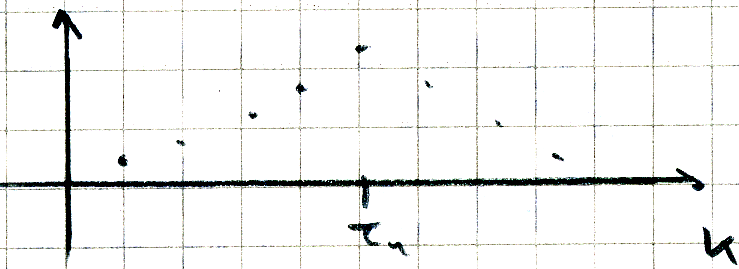
\includegraphics[width=1\textwidth]{./pics/MSTAT004.png}
		\caption{Plot von $\Earg{S_k}$}
		%\label{Abb}
	\end{center}
\end{figure}

Dies motiviert folgenden Schätzer (ersetze unbekannte $\abs[\big]{\Earg{S_k}}$ durch bekannte $\abs{S_k}$):
\begin{align*}
	\hat{τ}_n:=\argmax_{0≤ k≤ n}\abs[\big]{S_k}
\end{align*}
Im Folgenden sei $τ_n=\floor{ n·θ},θ∈(0,1)$.
Wir zeigen:
\begin{align*}
	\hat{θ}_n := \frac{\hat{τ}_n}{n} \ntoinf θ \qquad \P \text{-f.\,s.}
\end{align*}

\define{Annahme:} Wir nehmen die sogenannte \define{Momentenbedingung an}, d.\,h.
\begin{align*}
	μ_p := \Earg[\Big]{ \abs[\big]{X_{τ_n}}^p } < ∞,
	\qquad
	ν_p := \Earg[\Big]{ \abs[\big]{X_{τ_n+1}}^p } < ∞
\end{align*}

Sei $M_n:=$ der Polygonzug durch $\klammern{\frac{k}{n},\frac{1}{n} S_k}$, $0 ≤ k ≤ n$.
Dann folgt aus Lemma \ref{lemma7.17}:
\begin{align*}
	\hat{θ}_n&:=\argmax_{0≤ t≤ 1}\abs[\big]{M_n(t)}\\
	M_n(t) &= \frac{1}{n} S_{\floor{n t}}
	+ \klammern[\big]{n t - \floor{w t}}
	\klammern{ S_{\floor{n t} + 1} - S_{\floor{n t}}} & ∀\, 0 ≤ t ≤ 1 \\
	\Earg{M_n(t)} &=\frac{1}{n} \Earg{ S_{\floor{n t}}} + \klammern{n t - \floor{w t}}
	\klammern{\Earg{S_{\floor{n t} + 1}} - \Earg{S_{\floor{n t}}} } & ∀\, 0 ≤ t ≤ 1 \\
\end{align*}

Sei $\overline{M}_n(t) := \Earg{M_n(t)}$, $0 ≤ t ≤ 1$.
Dann ist $\overline{M}_n$ ein Polygonzug durch die Punkte $\klammern{\frac{k}{n}, \frac{1}{n} \Earg{S_k}}$, $0 ≤ k ≤ n$.
Da wegen \eqref{eqUnder8.2_1}
\begin{align*}
	\overline{M}_n\klammern{\frac{k}{n}}
	&=\frac{1}{n} \Earg[\big]{S_k}
	\overset{\eqref{eqUnder8.2_1}}
	=
	\begin{cases}
		\frac{k}{n} (1-θ_n) (μ-ν) &\falls \frac{k}{n} ≤ \frac{τ_n}{n} = θ_n\\
		\klammern{1-\frac{k}{n}} θ_n (μ-ν), & \falls \frac{k}{n} > θ_n
	\end{cases}
\end{align*}
folgt
\begin{align*}
	\overline{M}_n\klammern{t}
	&=
	\begin{cases}
		t (1 - θ_n) (μ-ν) & \falls t ≤ θ_n \\
		\klammern{1-t} θ_n (μ-ν), & \falls \frac{k}{n} > θ_n
	\end{cases}
\end{align*}
Beachte $θ - \frac{1}{n} < θ_n = \frac{\floor{nθ}}{n} \leq θ$.
Eine Fallunterscheidung ($t≤θ_n$; $θ_n<t≤θ$; $t>θ$) liefert
% θ_n > θ → größte Unterschiede möglich bei θ und θ_n
% alles ·(μ - ν) im Folgenden
% bei θ: θ(1-θ) - θ(1-θ_n) = Θ(θ_n - θ) < θ/n
% bei θ_n: θ_n(1-θ_n) - (1-θ_n)θ = (1-θ_n)(θ_n - θ) < (1-θ_n)/n
% → da könnte auch 1 statt 2 stehen, aber gut, 2 > 1
\begin{align}\label{eqUnder8.2_2}\tag{2}
	\norm[\big]{\overline{M}_n-M}
	&= \sup_{0 ≤ t ≤ 1} \abs[\Big]{\overline{M}_n(t) - M(t)}
	≤ \frac2n \abs{μ-ν} \ntoinf 0 \text{, wobei} \\ \nonumber
	M(t) &=
	\begin{cases}
		t (1-θ) (μ-ν) , & \falls 0 ≤ t ≤ θ\\
		(1-t) θ (μ-ν), & \falls θ < t ≤ 1
	\end{cases}
	\\ \nonumber
	\abs{M(t)} &=
	\begin{cases}
		t (1-θ) \abs{μ-ν} , & \falls 0 ≤ t ≤ θ \\
		(1-t) θ \abs{μ-ν} , & \falls θ < t ≤ 1
	\end{cases}
\end{align}

\begin{figure}[H]
	\begin{center}
		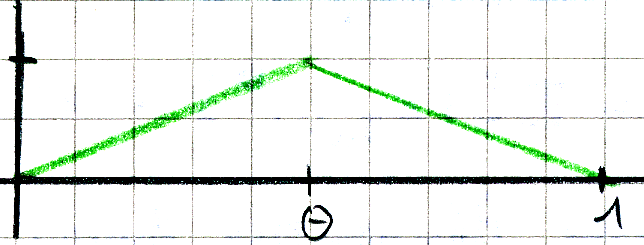
\includegraphics[width=1\textwidth]{./pics/MSTAT005.png}
		\caption{Plot von $M(t)$}
		%\label{AbbTitel}
	\end{center}
\end{figure}

Somit ist dieses $θ$ charakterisierbar als Maximalstelle:
\begin{align*}
	θ=\argmax_{0≤ t≤ 1}\abs[\big]{M(t)}
\end{align*}

Zeige:
\begin{align*}
	\norm[\big]{ M_n-M}
	&= \sup_{0 ≤ t ≤ 1} \abs[\big]{M_n(t)-M(t)} \ntoinf 0 \quad \P\text{-f.\,s.}
\end{align*}
Da
\begin{align}\label{eqUnder8.2_3}\tag{3}
	0≤\norm[\big]{ M_n-M}≤\norm[\big]{ M_n-\overline{M}_n}+\underbrace{\norm[\big]{\overline{M}_n-M}}_{
		\stackrelnew{\eqref{eqUnder8.2_2}}{n⟶∞}{\longrightarrow}0
	}
\end{align}

betrachte den ersten Summanden
\begin{align}\label{eqUnder8.2_4}\tag{4}
	\norm[\big]{M_n - \overline{M}_n}
	= \sup_{0 ≤ t ≤ 1} & \abs[\big]{M_n(t) - \overline{M}_n(t)}
	\overset{\ref{lemma7.17}}{=}
	\max_{0 ≤ k ≤ n} \abs[\bigg]{\underbrace{
			M_n \argu{\frac{k}{n}}
		}_{= \frac{1}{n} S_k}
		- \underbrace{
			\overline{M}_n \argu{\frac{k}{n}}
		}_{=\frac{1}{n} \Earg{S_k}}
	} \\
	\nonumber
	\frac{1}{n} S_k
	&= \frac{1}{n} \sum_{i=1}^k\klammern[\big]{X_i - \overline{X}_n}
	= \frac{1}{n} \sum_{i=1}^k X_i - \frac{k}{n^2} \sum_{i=1}^n X_i \\ \nonumber
	⇒
	M_n \argu{\frac{k}{n}} - \overline{M}_n \argu{\frac{k}{n}}
	\overset{\text{Lin}}&=
	\frac{1}{n} \sum_{i=1}^k \underbrace{
		\klammern[\Big]{X_i - \Earg[\big]{X_i}}
	}_{=:Z_i}
	- \frac{k}{n^2} \sum_{i=1}^n \underbrace{
		\klammern[\Big]{X_i - \Earg[\big]{X_i}}
	}_{=Z_i} \\ \nonumber
	⇒
	\abs{M_n \argu{\frac{k}{n}} - \overline{M}_n \argu{\frac{k}{n}}}
	\overset{\laplace\neq}&{≤}  % laplace is a triangle % Dreiecksungleichung
	\frac{1}{n} \underbrace{
		\abs[\bigg]{\sum_{i=1}^k
			\klammern[\big]{X_i - \Earg[\big]{X_i}}
		}
	}_{
		≤ \max_{0 ≤ k ≤ n} \abs{\sum_{i=1}^k Z_i}
	} + \underbrace{
		\frac{k}{n^2}
	}_{≤\frac{1}{n}}
	\underbrace{
		\abs[\bigg]{\sum_{i=1}^n
			\klammern[\Big]{X_i - \Earg[\big]{X_i}}
		}}_{
			≤\max_{0 ≤ k ≤ n} \abs{\sum_{i=1}^k Z_i}
		} \\ \nonumber
		&≤ \frac{2}{n} \max_{0 ≤ k ≤ n} \abs{\sum_{i=1}^k Z_i}\\
	⇒\label{eqUnder8.2_5}\tag{5}
	& \max_{0 ≤ k ≤ n} \abs{M_n \argu{\frac{k}{n}} - \overline{M}_n \argu{\frac{k}{n}}}
	≤ \frac{2}{n} \max_{0 ≤ k ≤ n} \abs{\sum_{i=1}^k Z_i}
\end{align}

Es ist
\begin{align*}
	T_k=\sum_{i=1}^k Z_i\qquad 0≤ k≤ n
\end{align*}
ein Martingal bzgl.\ der Filtration
\begin{align*}
	\F_k:=σ\klammern[\big]{Z_1,…,Z_k} &\qquad∀ 1≤ k≤ n,\qquad \F_0:=\set{∅,Ω}
\end{align*}
Es ist Martingal, weil
\begin{align*}
	\Earg{T_{k+1}~\middle|~\F_k}
	% CHECKED: '|' used.
	&=\Earg{\klammern{\sum_{i=1}^k Z_i} + Z_{k + 1} ~ \middle| ~ \F_k}
	% CHECKED: '|' used.
	= \underbrace{
		\Earg[\bigg]{ \overbrace{\sum_{i=1}^k Z_i}^{\text{ist $\F_K$-messbar}}
		~\bigg|~ \F_k}
		% CHECKED: '|', '\bigg' used.
	}_{ = T_k}
	% CHECKED: '\bigg' used
	+ \underbrace{\Earg{ Z_{k + 1}~\middle|~\F_k}}_{= \Earg{Z_{k + 1}} = 0}
	% CHECKED: '|' used.
\end{align*}

Es folgt aus der bedingten Jensenungleichung, dass $\klammern{\abs{T_k}^p,\F_k}_{0≤ k≤ n}$ ein nicht-negatives Submartingal ist.
\begin{align}\nonumber
	\P\argu{\norm[\big]{M_n - \overline{M}_n} ≥ ε}
	\overset{\eqref{eqUnder8.2_4}+\eqref{eqUnder8.2_5}}&{≤}
	\P \argu{ \frac{2}{n} \max_{0 ≤ k ≤ n} \abs[\big]{T_k} \geq ε } \\ \nonumber
	&≤ \P\argu{\max_{0 ≤ k ≤ n} \abs[\big]{T_k} ≥ \frac{1}{2} n ε} \\ \nonumber
	\overset{u↦ u^p\uparrow}&{=}
	% tocheck: im original war hier ein \leq statt =, aber es sollte doch = sein, oder?
	% ist auch egal, da eh abgeschätzt wird
	\P \argu{\klammern{\max_{0 ≤ k ≤ n} \abs[\big]{T_k}}^p ≥ \klammern{\frac{1}{2} n ε}^p} \\ \nonumber
	&= \P \argu[\bigg]{\max_{0 ≤ k ≤ n} \underbrace{
		\abs[\big]{T_k}^p
	}_{\text{Submartingal}}
	≥ \underbrace{
		\klammern{\frac{1}{2} nε}^p
	}_{=: y > 0}} \\ \nonumber
	% ⇒
	% \P \argu{\norm[\big]{ M_n - \overline{M}_n} ≥ ε}
	% &≤ \P\argu[\bigg]{\max_{0 ≤ k ≤ n} \underbrace{
		% \abs[\big]{T_k}^p
	% }_{\text{Submartingal}} ≥ \underbrace{2^{-p}· n^p·ε^p}_{=:y>0}} \\ \nonumber
	\overset{\text{Doob-Ungl\footnotemark}}&{≤}
	% footnotetext later
	y^{-1} \Earg{\abs{T_n}^p}\\
	&= 2^p n^{-p} ε^{-p} \Earg{ \abs{ \sum_{i=1}^n Z_i }^p } \label{eqUnder8.2_6} \tag{6}
\end{align}
% see Kopka and Daly, A Guide to LaTeX, p. 96--97: never put footnotes in math env
% or see https://tex.stackexchange.com/questions/21813/footnote-in-math-mode for this solution
% fix still necessary: link jumps to first page
\footnotetext{Siehe \url{https://de.wikipedia.org/wiki/Doobsche_Maximalungleichung}}
Es gilt folgende \define{Momenten-Ungleichung} (vergleiche \cite[(1.6), Seiten 96 bis 101]{ferger2014optimal})% (1.6) in Ferger (2014), \undefine{Optimal constants in the Marcinkiewicz-Zygmund-inequalities, statistics and propability letters} Ausgabe 84, Seiten 96 bis 101)

\begin{align*}
	\Earg{ \abs{ \sum_{i=1}^n Z_i }^p }
	\overset{\text{\cite[1.6]{ferger2014optimal}}}{≤}
	C_p n^{\frac{p}{2}} \sum_{i=1}^n \Earg{\abs{Z_i}^p}
\end{align*}

Erinnerung:
\begin{align*}
	Z_i&=X_i-\Earg{X_i}\\
	⇒
	\abs{Z_i}^p&=\abs[\big]{X_i-\Earg{X_i}}^p\\
	⇒
	\abs[\big]{X_i-\Earg{X_i}}^p
	\overset{\eqref{eqCrUngleichung}%C_r\text{ Ungl}
	}&{≤}
	c_p \klammern[\Big]{
		\abs{X_i}^p
		+ \underbrace{
			\abs[\big]{\Earg{X_i}}^p}_{
				\overset{\text{Jensen}}{≤} \Earg[\big]{\abs{X_i}^p}
		}
	} \\
	⇒
	\Earg[\Big]{\abs{Z_i}^p}
	&≤ c_p \klammern{\Earg[\big]{\abs{X_i}^p} + \Earg[\big]{\abs{X_i}^p}} \\
	&≤ 2 c_p \Earg[\Big]{\abs{X_i}^p}
	≤ 2 c_p \max \set{μ_p, ν_p}
\end{align*}
Somit gibt es eine Konstante $D_p$ so, dass
\begin{align*}
	\Earg{\abs{\sum_{i=1}^n Z_i}^p}
	\overset{\text{\cite[(1.6)]{ferger2014optimal}}}&{≤}
	C_p n^{\frac{p}{2}} \sum_{i=1}^n \underbrace{\Earg[\Big]{\abs{Z_i}^p}}_{≤ D_p} \\
	⇒
	\Earg{ \abs{ \sum_{i=1}^n Z_i }^p }
	&≤ \tilde{c}_p · n^{\frac{p}{2}} \\
	\overset{\eqref{eqUnder8.2_6}}{⇒}
	\P\argu{ \norm[\big]{M_m - \overline{M}_n} ≥ ε }
	&≤ \overline{c}_p n^{-\frac{p}{2}} ε^{-p} \qquad ∀ ε > 0
\end{align*}

Nun bilden wir die Reihe dieser Wahrscheinlichkeiten und erhalten Konvergenz für $p>2$:
\begin{align*}
	\overset{p>2}{⇒}
	\sum_{n=1}^∞ \P\argu{\norm[\big]{M_m - \overline{M}_n} ≥ ε } < ∞ \qquad ∀ ε > 0
\end{align*}

Es gilt ganz allgemein für eine Folge $(ζ_n)_{n∈ℕ}$ von Zufallsvariablen (folgt aus dem Borel-Cantelli-Lemma):
\begin{align*}
	\klammern{∀ ε > 0 : \sum_{n=1}^∞ \P\argu[\Big]{\abs{ζ_n} ≥ ε} < ∞ } ⇒ ζ_n \ntoinf 0 \text{ f.\,s.}
\end{align*}

Also erhalten wir
\begin{align*}
	\norm[\big]{M_n - \overline{M}_n} \ntoinf 0 \text{ f.\,s.} \\
	\overset{\eqref{eqUnder8.2_2}+\eqref{eqUnder8.2_3}}{⇒}
	\norm[\big]{M_n - M} \ntoinf 0 \text{ f.\,s.}
\end{align*}

Da
\begin{align*}
	\norm[\Big]{\abs[\big]{M_n}-\abs[\big]{M}} ≤ \norm{M_n - M}
\end{align*}
folgt
\begin{align*}
	\norm[\Big]{ \abs[\big]{M_n} - \abs[\big]{M} } \overset{n⟶∞}&{\longrightarrow} 0 \text{ f.\,s.}\\
	⇒
	\norm[\Big]{- \abs[\big]{M_n} - \klammern[\big]{ -\abs[\big]{M} } } \overset{n⟶∞}&{\longrightarrow} 0 \text{ f.\,s.}\\
	% ⇒
	\hat{θ}_n
	&=\argmax_{0≤ t≤ 1}\abs[\big]{M_n(t)}
	=\argmin_{0≤ t≤ 1}-\abs[\big]{M_n(t)}
\end{align*}
Also hat $-\abs{M}$ eindeutige Minimalstelle $θ$.
% todo: warum folgt die eindeutigkeit daraus? Sollte die nicht aus der Hut-fkt-def von oben folgen?
Aus Satz \ref{satz8.6} folgt nun $\hat{θ}\ntoinf θ$ f.\,s..
(In Satz \ref{satz8.6} verwende: $M_n\hat{=}-\abs{M_n}$, $M\hat{=} - \abs{M}$, $τ \hat{=} θ$.)

\begin{bemerkung}
	Betrachte eine endliche Beobachtungsfolge:
	\begin{equation*}
		X_1, X_2, …, X_τ, X_{τ+1}, X_{τ+2}, …, X_n \qquad n > τ \\
	\end{equation*}
	Hier braucht man keinen doppelten Index.
	Vergrößert man aber nun $n$, dann geht der Anteil an der Gesamtstichprobe gegen $0$, also $\frac{τ}{n} → 0$.
\end{bemerkung}

Zusammenfassung unserer Überlegungen in
\begin{satz}\label{satz8.7} % in WiSe 2018/19: Satz 8.8
	Sei $θ∈(0,1)$, $μ \neq ν$, $μ_p < ∞$, $ν_p < ∞$ für ein $p > 2$.
	Dann gilt:
	\begin{align*}
		\hat{θ}_n
		&= \frac{1}{n} \underbrace{
			\argmax_{0 ≤ k ≤ n} \abs{ \sum_{i=1}^k \klammern[\big]{X_i - \overline{X}_n}}
		}_{= \hat{τ}_n} \ntoinf 0 \text{ f.\,s.}
	\end{align*}
\end{satz}

\begin{bemerkung}
	% todo: zusätzliche Bemerkung
	 Es gilt \emph{nicht}, dass $\hat{τ}_n - τ_n \ntoinf 0$ f.\,s..
	 Tatsächlich gilt:
	 \begin{align*}
	 	\hat{τ}_n-τ_n\distrto  T
	 \end{align*}
	 wobei $T$ die f.\,s.\ eindeutige Maximalstelle einer \undefine{2-seitigen Irrfahrt / Random Walk} auf $\Z$ ist
	 (vergleiche \cite[Seiten 362 bis 378]{ferger1994asymptotic}). %D.F. (1994) \undefine{Asymptotic distribution theory of change-point estimators} veröffentlicht in \undefine{Mathematical methods in statics 3}, Seiten 362 bis 378).
\end{bemerkung}


